% Dmitry Mikushin, UNIL, dmitry@kernelgen.org

\documentclass[aspectratio=169,twoside]{beamer}

\usetheme{unil}
\usepackage{comment}
\usepackage{enumerate}
\usepackage{xcolor}
\usepackage{setspace}
\usepackage{mathrsfs}
\usepackage{multibbl}
\usepackage{relsize}
\usetikzlibrary{calc,shapes.callouts,shapes.arrows}

\title[HPC Multi-iterator Engine]{HPC Multi-iterator Engine\\ Design \& Implementation}
\author[Dmitry Mikushin et al.]{Dmitry Mikushin\quad Simon Scheidegger\\ Philipp Eisenhauer\quad Moritz Mendel}
\institute[UNIL]{}
\date{May 4, 2021}



\begin{document}



{
\setbeamertemplate{footline}{} 
\begin{frame}
  \titlepage
\end{frame}
}
\addtocounter{framenumber}{-1}



\setbeamercovered{transparent=5}



\begin{frame}[fragile]{Multi-Iterator: the purpose}

\begin{center}
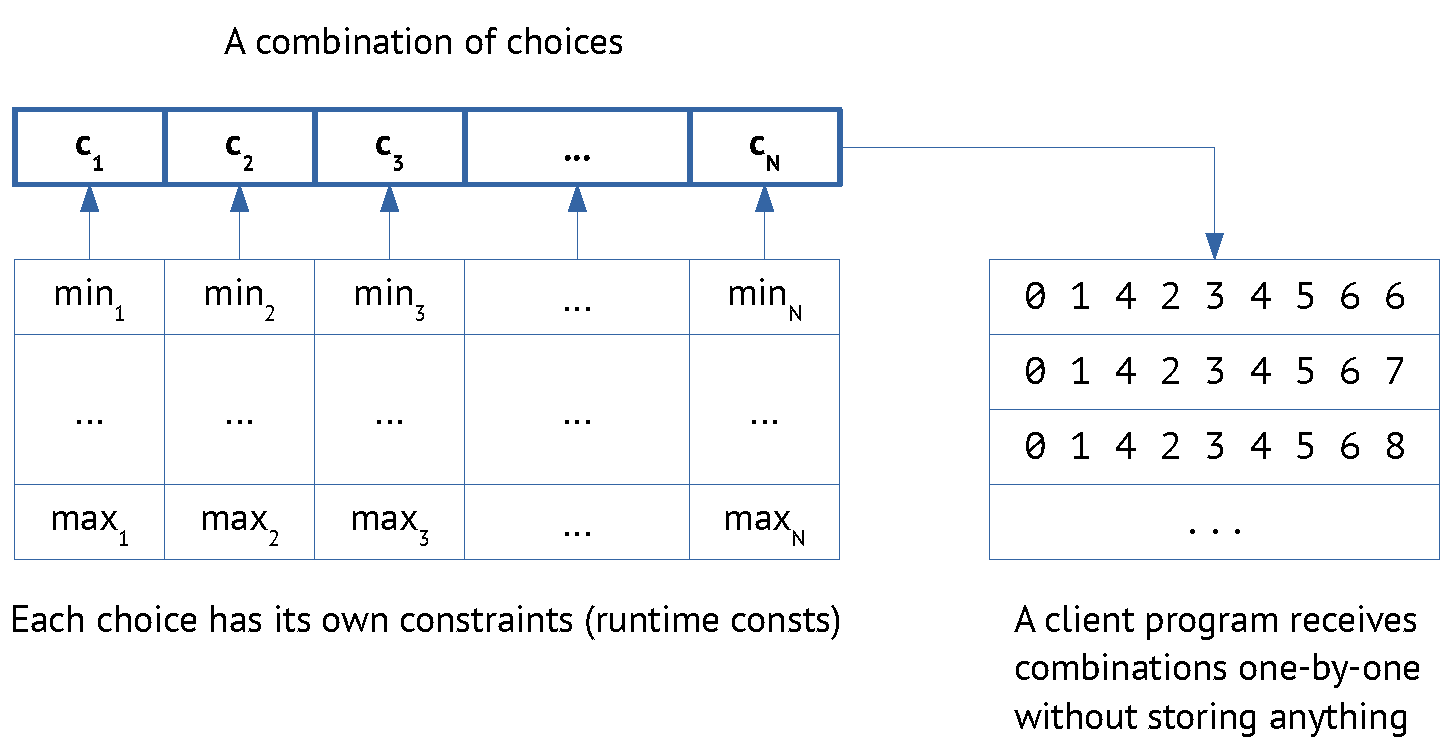
\includegraphics[width=11cm]{figures/combinations}
\end{center}

\end{frame}



\begin{frame}[fragile]{Multi-Iterator: motivation}

Three horrible ways to implement a multi-iterator:

\begin{itemize}
\item Store a matrix of all combinations in RAM (slow, only small problems could fit in)
\item Generate combinations recursively (non-parallel)
\item Implement bounds check with \texttt{if..else} (pipeline stalls)
\end{itemize}

\vskip10pt

Three optimization ideas for high-performance multi-iterator:

\begin{itemize}
\item On-the-fly generation (and use) of combinations (no memory penalty)
\item Use JIT-compliation (trending in modern HPC, see \href{https://www.youtube.com/watch?v=6dv9vdGIaWs&ab_channel=CppCon}{ClangJIT talk by Hal Finkel})
\item Use predicates (bitmasks) instead of branching
\end{itemize}

\end{frame}



\begin{frame}[fragile]{Simple example}

\begin{minipage}{9cm}
\begin{lstlisting}[basicstyle=\tiny\ttfamily, language=c++]
#include <multiit/multiit.h>

int main(int argc, char* argv[])
{
    multiit::runtime::MultiIterator mi({ 2, 3, 4 }); 
    // OR: multiit::compiletime::MultiIterator<2, 3, 4> mi; 

    int niters = 0;
    const int size = mi.getSize();
    while (1) 
    {   
        niters++;
        if (!mi.next()) break;

        // TODO Use the current combination of choices in a target app.
        const auto& current = mi.getCurrent();
        for (int i = 0; i < size; i++)
            printf("%d ", current[i]);
        printf("\n");
    }   

    printf("%d iterations visited\n", niters);

    return 0;
}
\end{lstlisting}
\end{minipage}%
\begin{minipage}{0.5cm}
\hskip0.5cm
\end{minipage}%
\begin{minipage}{5cm}
\begin{lstlisting}[basicstyle=\tiny\ttfamily]
./multiit_example                     
1 0 0 
0 1 0 
1 1 0 
0 2 0 
1 2 0 
0 0 1 
1 0 1 
0 1 1 
1 1 1 
0 2 1 
1 2 1 
0 0 2 
1 0 2 
0 1 2 
1 1 2 
0 2 2 
1 2 2 
0 0 3 
1 0 3 
0 1 3 
1 1 3 
0 2 3 
1 2 3 
24 iterations visited
\end{lstlisting}
\end{minipage}

\end{frame}



\begin{frame}[fragile]{Supported types of multi-iterators}

\begin{itemize}
\item \texttt{MultiIterator}: A group of indexes that iterate from 0 to the given upper value
\item \texttt{LimitedMultiIterator}: A group of indexes that iterates only through indexes with total sum no greater than limit
\item \texttt{GenericMultiIterator}: A hosting group of indexes, whose indexes are themselves groups of indexes
\end{itemize}

\vskip20pt

$\Rightarrow$ A \texttt{GenericMultiIterator} of \texttt{MultiIterator} and \texttt{LimitedMultiIterator} elements can be used to express many kinds of combinatorial iterations

\end{frame}



\begin{frame}[fragile]{Programming package structure}

\begin{itemize}
\item \texttt{multiit}: general-purpose multi-iterators in C++, with unit tests
\item \texttt{kernit}: multi-iterator \emph{kernel} generator based on JIT-compilation located in the cloud (web service)
\item \texttt{respyit} : subjected multi-iterators, with Python API, which quiries \texttt{kernit} to provide a kernel with required specifics
\end{itemize}

\end{frame}



\begin{frame}[fragile]{Cloud serivce + end-user application pipeline}

TODO Pipeline figure

\end{frame}



\begin{frame}[fragile]{End-user example}

\begin{lstlisting}[basicstyle=\tiny\ttfamily, language=python]
import respyit

# TODO
\end{lstlisting}

\end{frame}



\end{document}

